\section{Frontend-Design}
Das Frontend für den Feasibility Check basiert auf der bereits implementierten Weboberfläche des \gls{REALIS}-Systems. Die Funktionalität des Feasibility Checks wird in die bestehende Webanwendung für den \glsentrylong{QM} integriert, sodass das Projekt nicht mehr an das \gls{RPT}-Labor übergeben werden muss, um den Check durchzuführen. Stattdessen ermöglicht das neue, automatisierte System dem \gls{QM}, die Machbarkeit der angelegten Tests eigenständig und ohne Laborunterstützung zu überprüfen.

Zunächst legt der \glsentrylong{QM} ein neues \gls{REALIS}-Projekt für das zu qualifizierende Produkt an. Dieses Projekt kann mit mehreren unterschiedlichen Tests versehen werden, wobei der Nutzer durch vorgefertigte Templates unterstützt wird, die häufig verwendete Testkonfigurationen und zugehörige Daten enthalten.

Nachdem das Projekt vollständig angelegt wurde, gelangt der Benutzer auf die Weboberfläche, wie in Abbildung \ref{fig:whole-page} dargestellt.

\begin{figure}[!htbp] 
    \centering 
    \makebox[\textwidth]{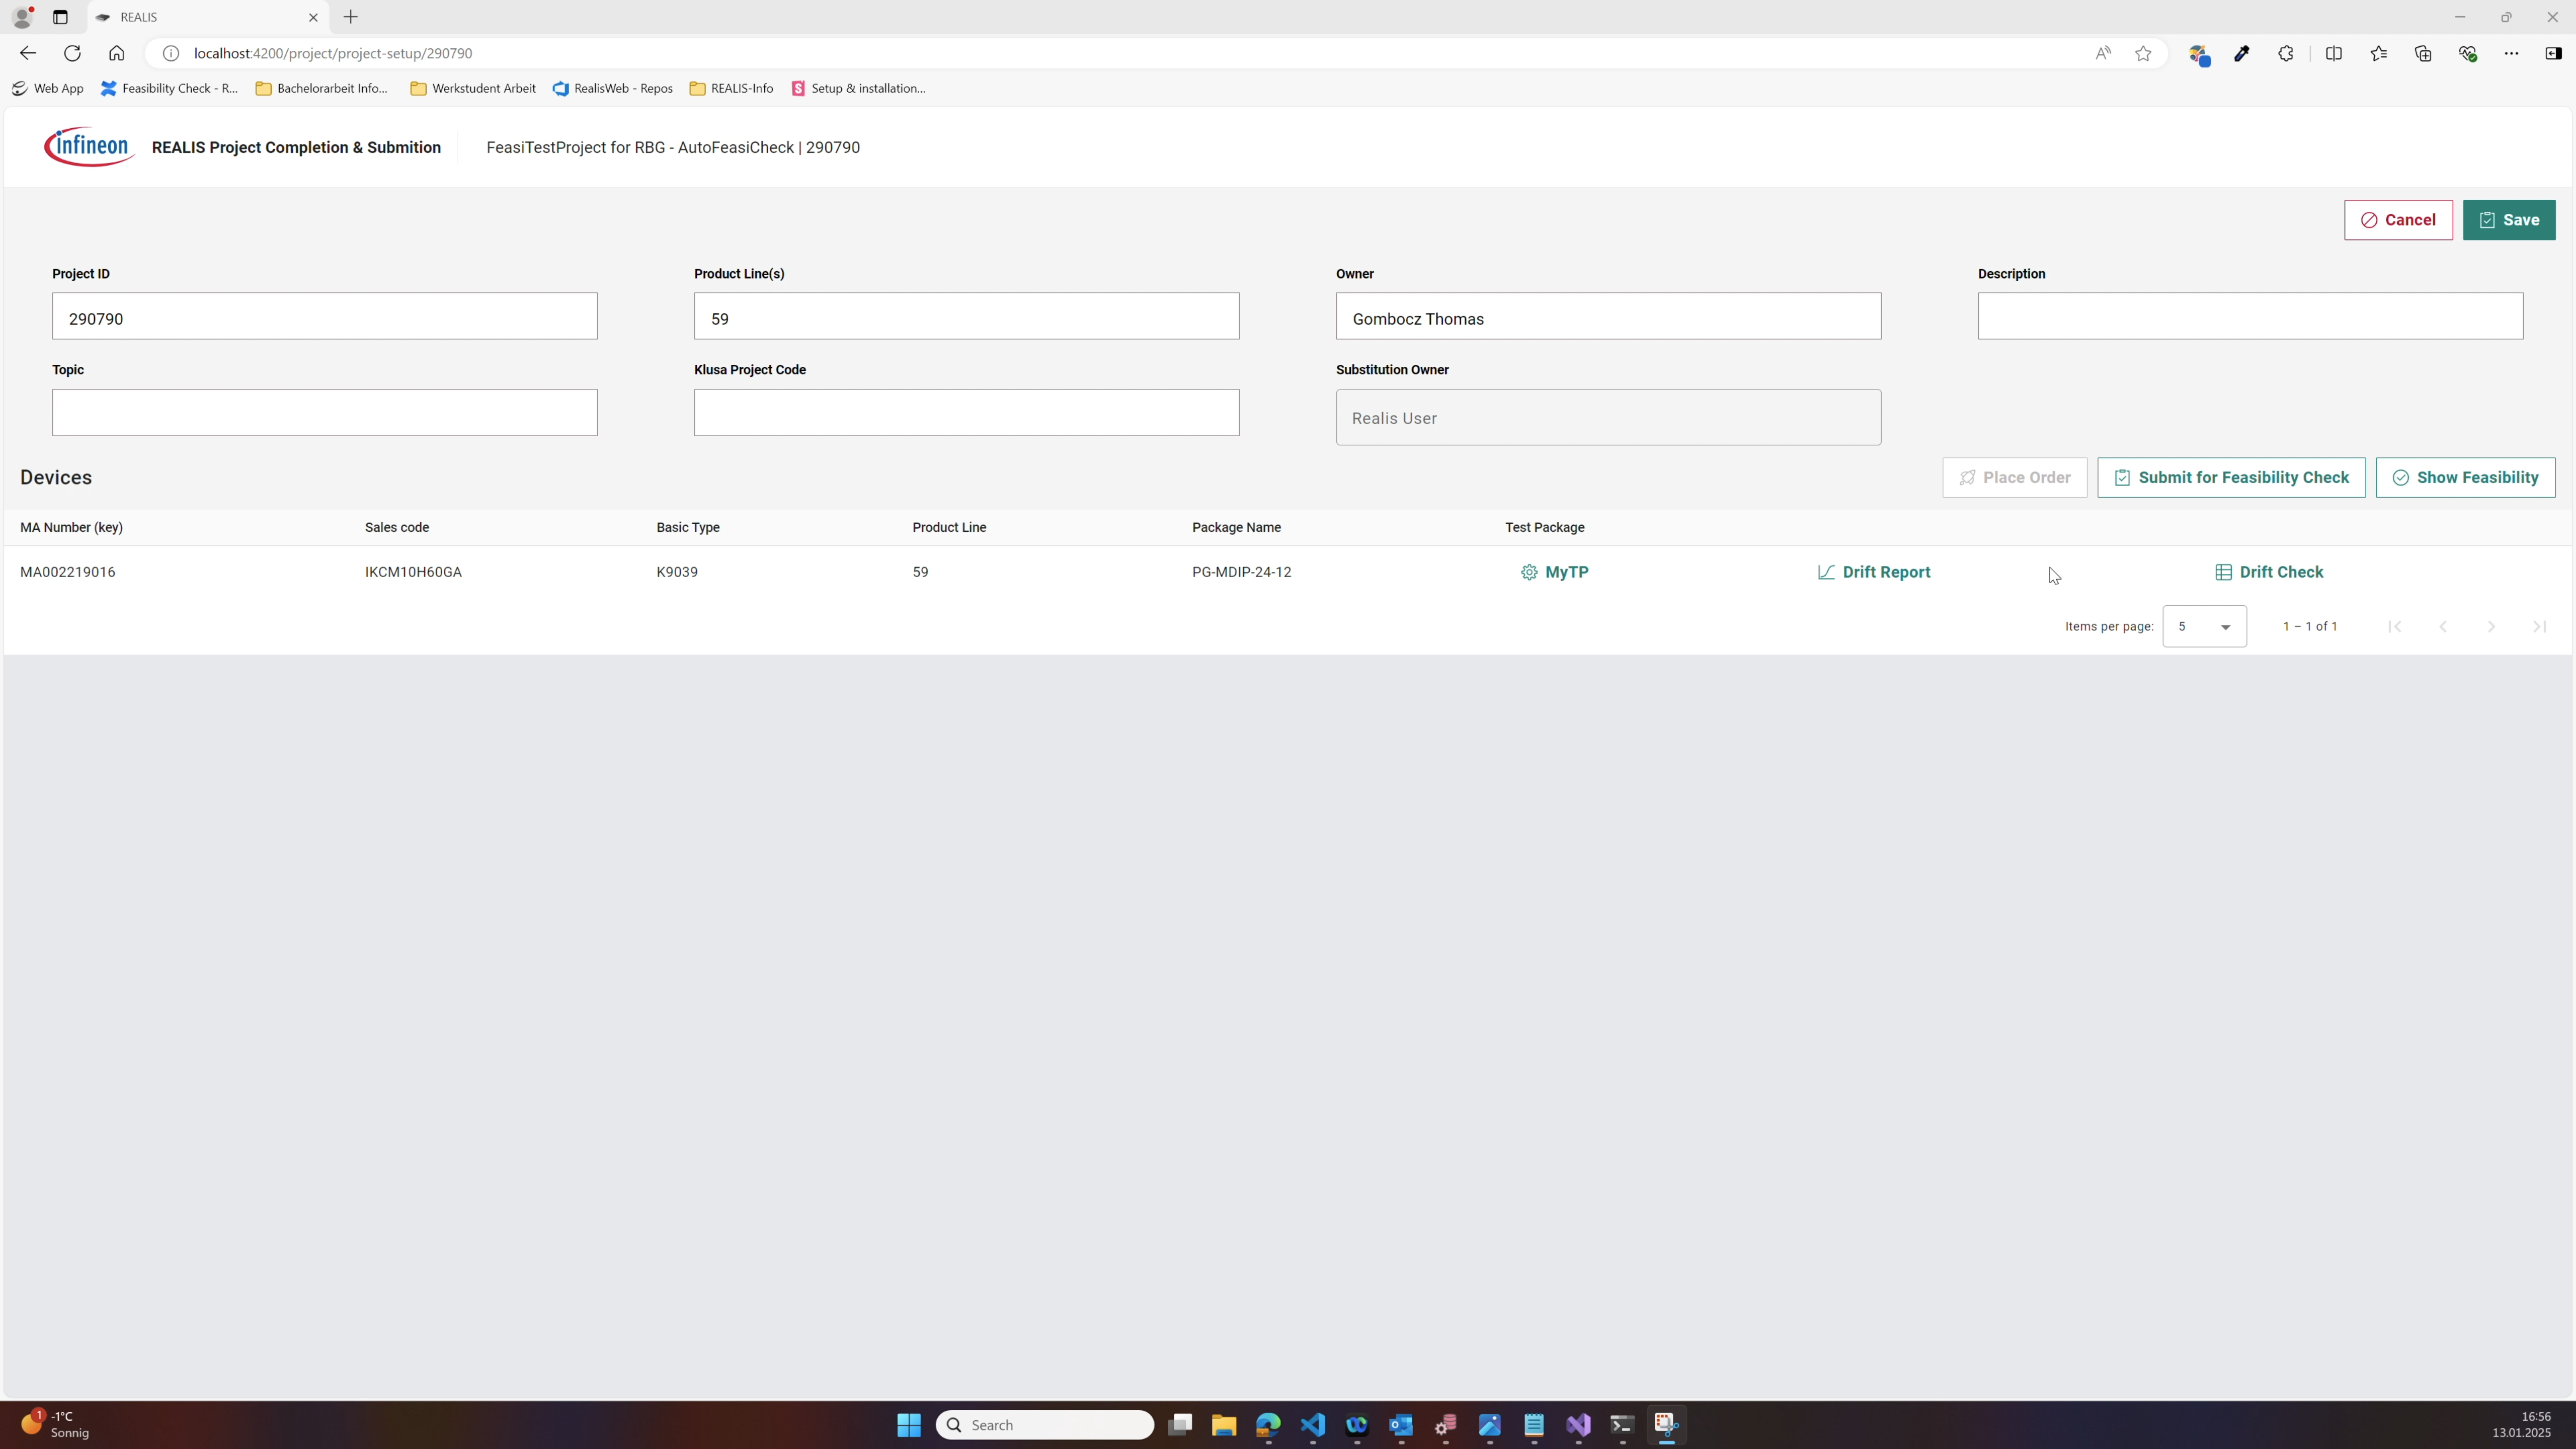
\includegraphics[width=0.85\paperwidth]{bilder/frontend/whole-page.png}} 
    \caption{Weboberfläche für den Quality Manager (QM) – Einstiegspunkt für den Feasibility Check} 
    \label{fig:whole-page} 
\end{figure}

Auf dieser Oberfläche kann der Feasibility Check für die definierten (Stress-)Tests durchgeführt werden. Auf der rechten Seite der Website befindet sich ein grün umrandeter Button mit der Beschriftung "Submit for Feasibility Check". Wird dieser Button betätigt, öffnet sich ein Popup-Fenster (Modal-Page), in dem dem Nutzer eine Übersicht der angelegten Tests in tabellarischer Form präsentiert wird. Diese Tabelle enthält die wichtigsten Informationen, wie den Teststatus und die eindeutige Test-ID (siehe Abbildung \ref{fig:submit-page}).

\subsection{Modal-Page für die Initiierung des Feasibility Checks}

In der Modal-Page können mittels CheckBoxen die einzelnen Tests ausgewählt werden, die den Feasibility Check durchlaufen sollen. Alternativ besteht die Möglichkeit, alle Tests gleichzeitig auszuwählen, indem die oberste CheckBox in der Spaltenüberschriftenleiste aktiviert wird (siehe Mauszeigerposition in Abbildung \ref{fig:submit-page}).

\begin{figure}[!htbp] 
    \centering 
    \makebox[\textwidth]{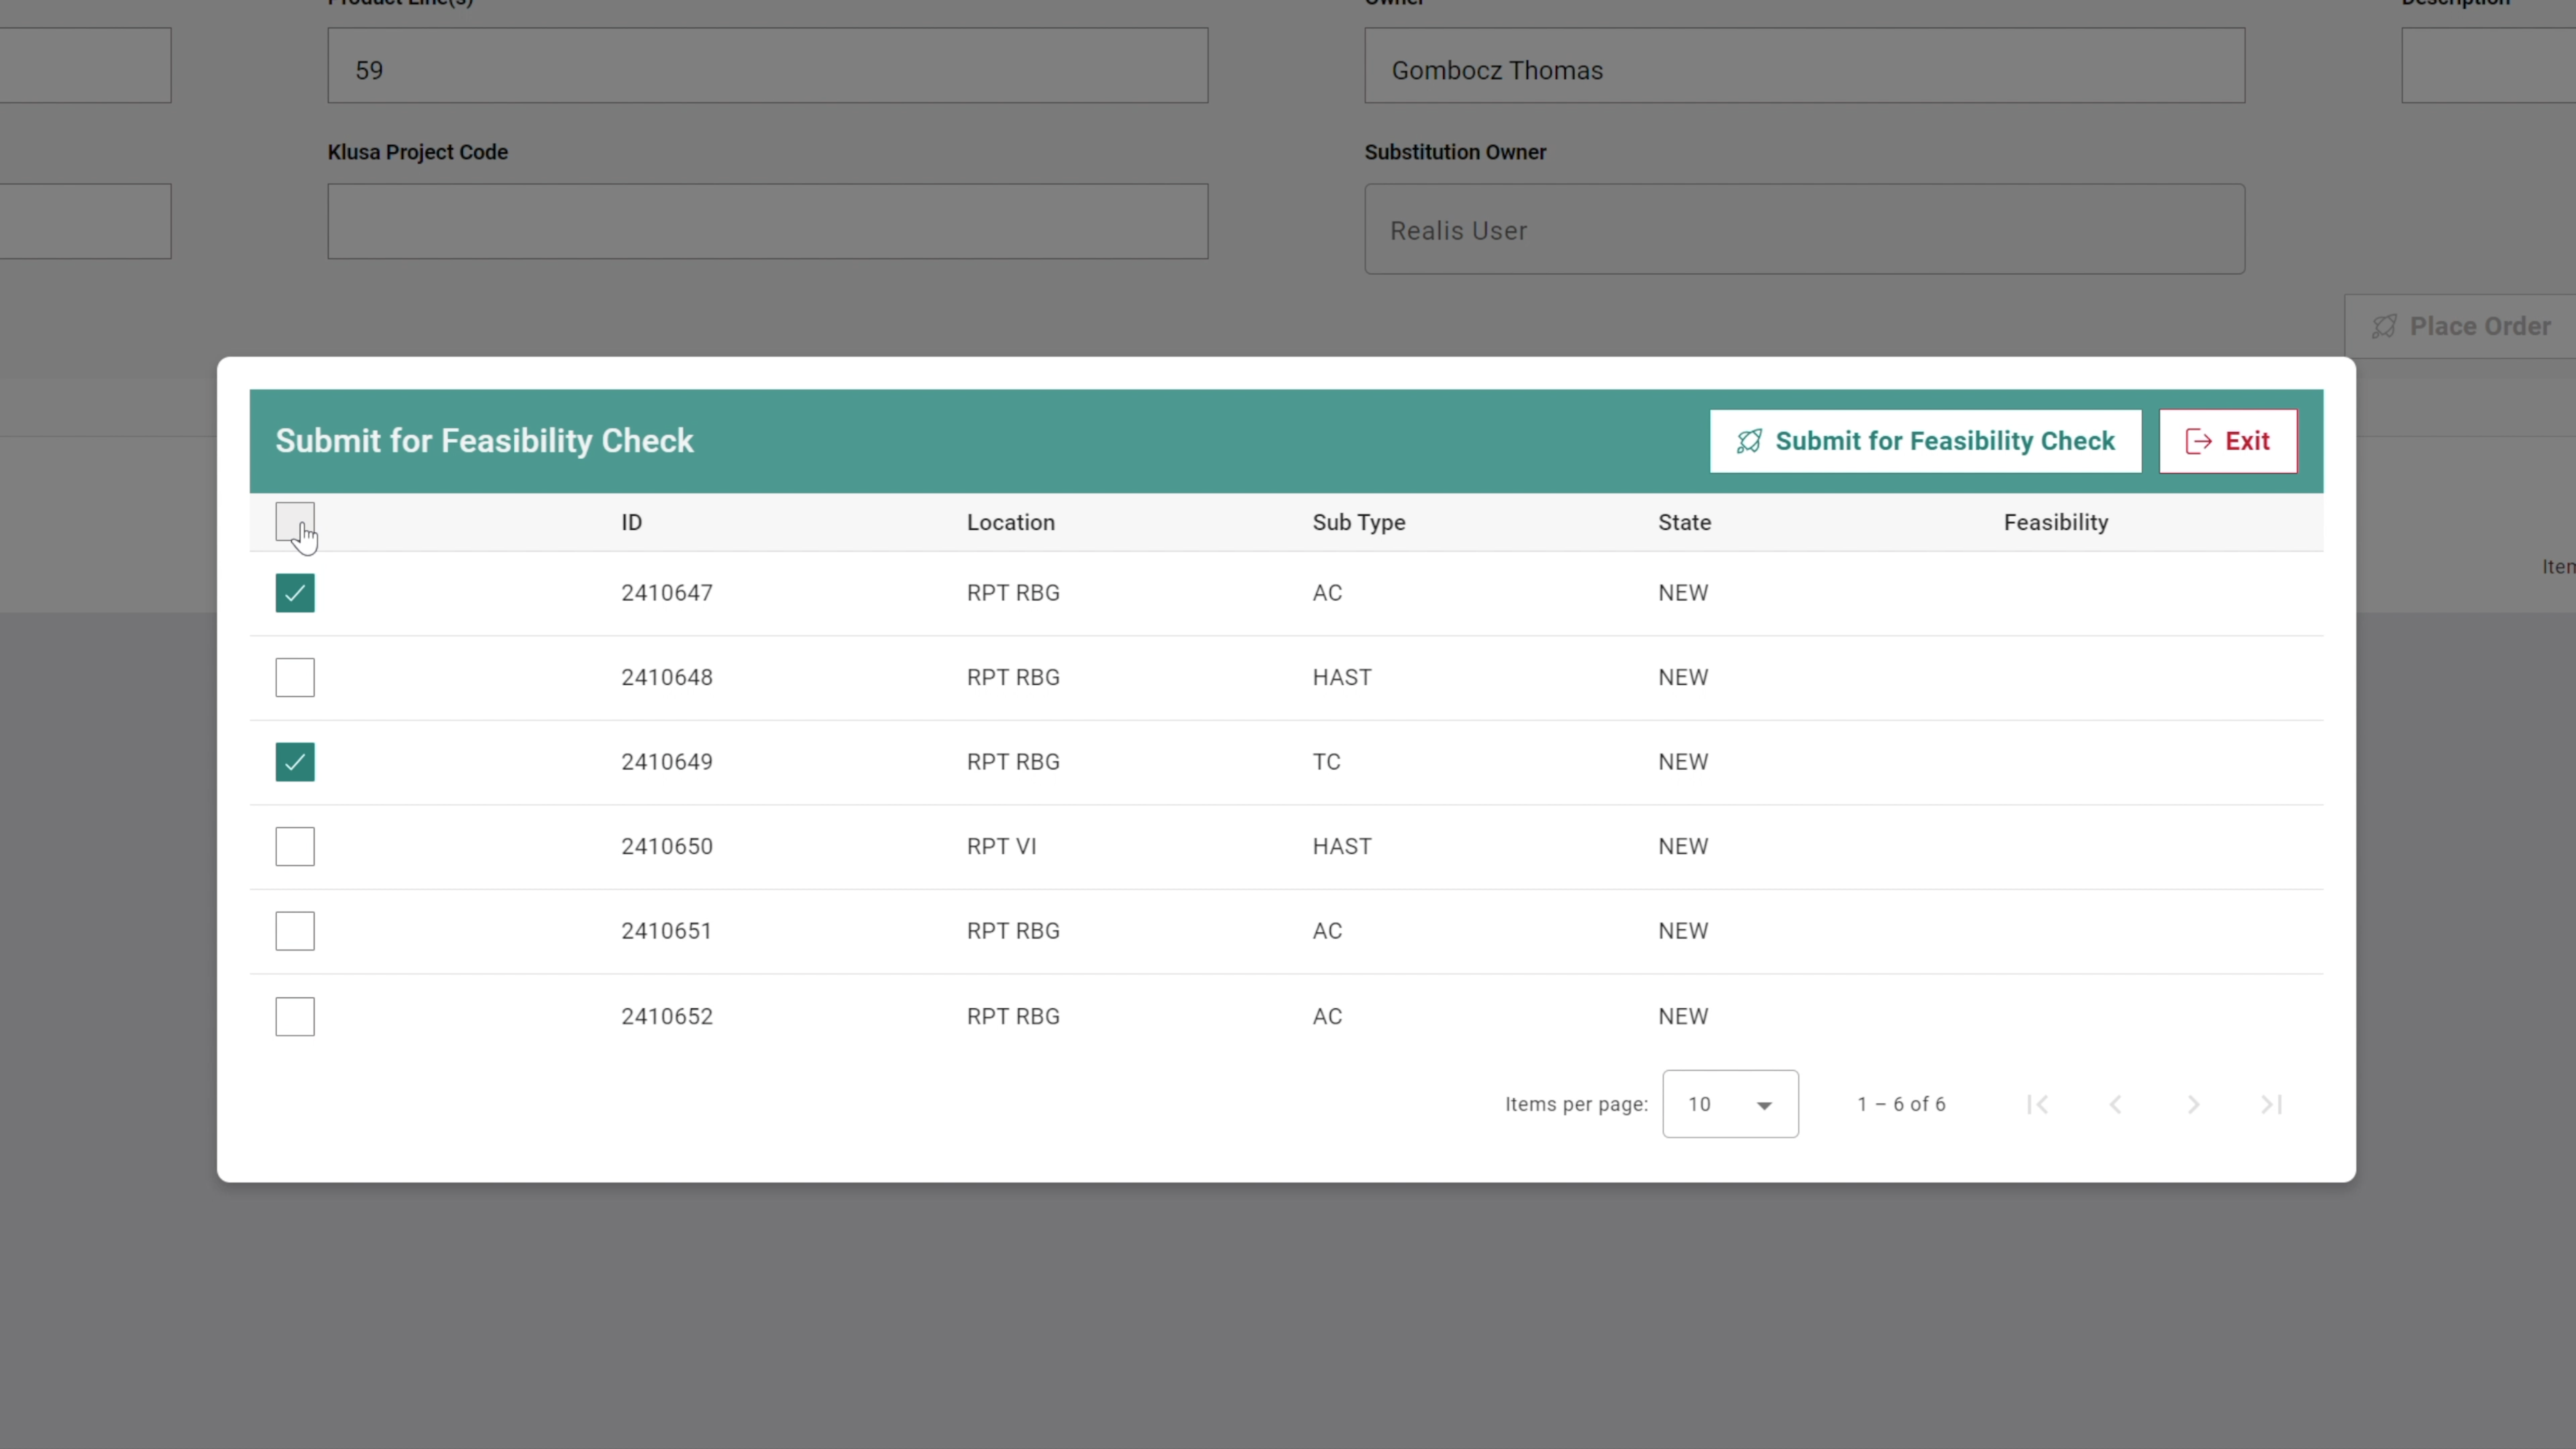
\includegraphics[width=0.85\paperwidth]{bilder/frontend/feasibility-modal-page.png}} 
    \caption{Modal-Page ''Submit for Feasibility Check'' – Modal-Page zur Initiierung des Feasibility Checks} 
    \label{fig:submit-page} 
\end{figure}

Nachdem der Benutzer die gewünschten Tests selektiert hat, klickt er auf den ''Submit for Feasibility Check''-Button, der oben links im Popup, neben dem ''Exit''-Button, positioniert ist. Mit diesem Klick wird für jeden ausgewählten Test ein asynchroner HTTP-Call an die Backend-Logik initiiert. Über die REST-API wird dabei die Helfer-Methode \texttt{CheckFeasibility()} aufgerufen, wobei die jeweilige Test-ID als Parameter übermittelt wird.

Die asynchronen HTTP-Calls ermöglichen es dem Benutzer, weiterhin mit der Oberfläche zu interagieren, während die Überprüfungen im Hintergrund durchgeführt werden. Dadurch kann der Benutzer das Popup schließen oder andere Aktionen ausführen, ohne den laufenden Feasibility Check zu unterbrechen. Die rotierenden Ladekreise in der "Feasibility"-Spalte rechts veranschaulichen den Ladevorgang für den Feasibility Check jedes Tests (siehe Abbildung \ref{fig:loading-with-results}). Bis ein Resultat eintrifft vergehen circa 2 bis 15 Sekunden, je nach Feasibility-Konfiguration und Komplexität des Tests.

\begin{figure}[!htbp] 
    \centering 
    \makebox[\textwidth]{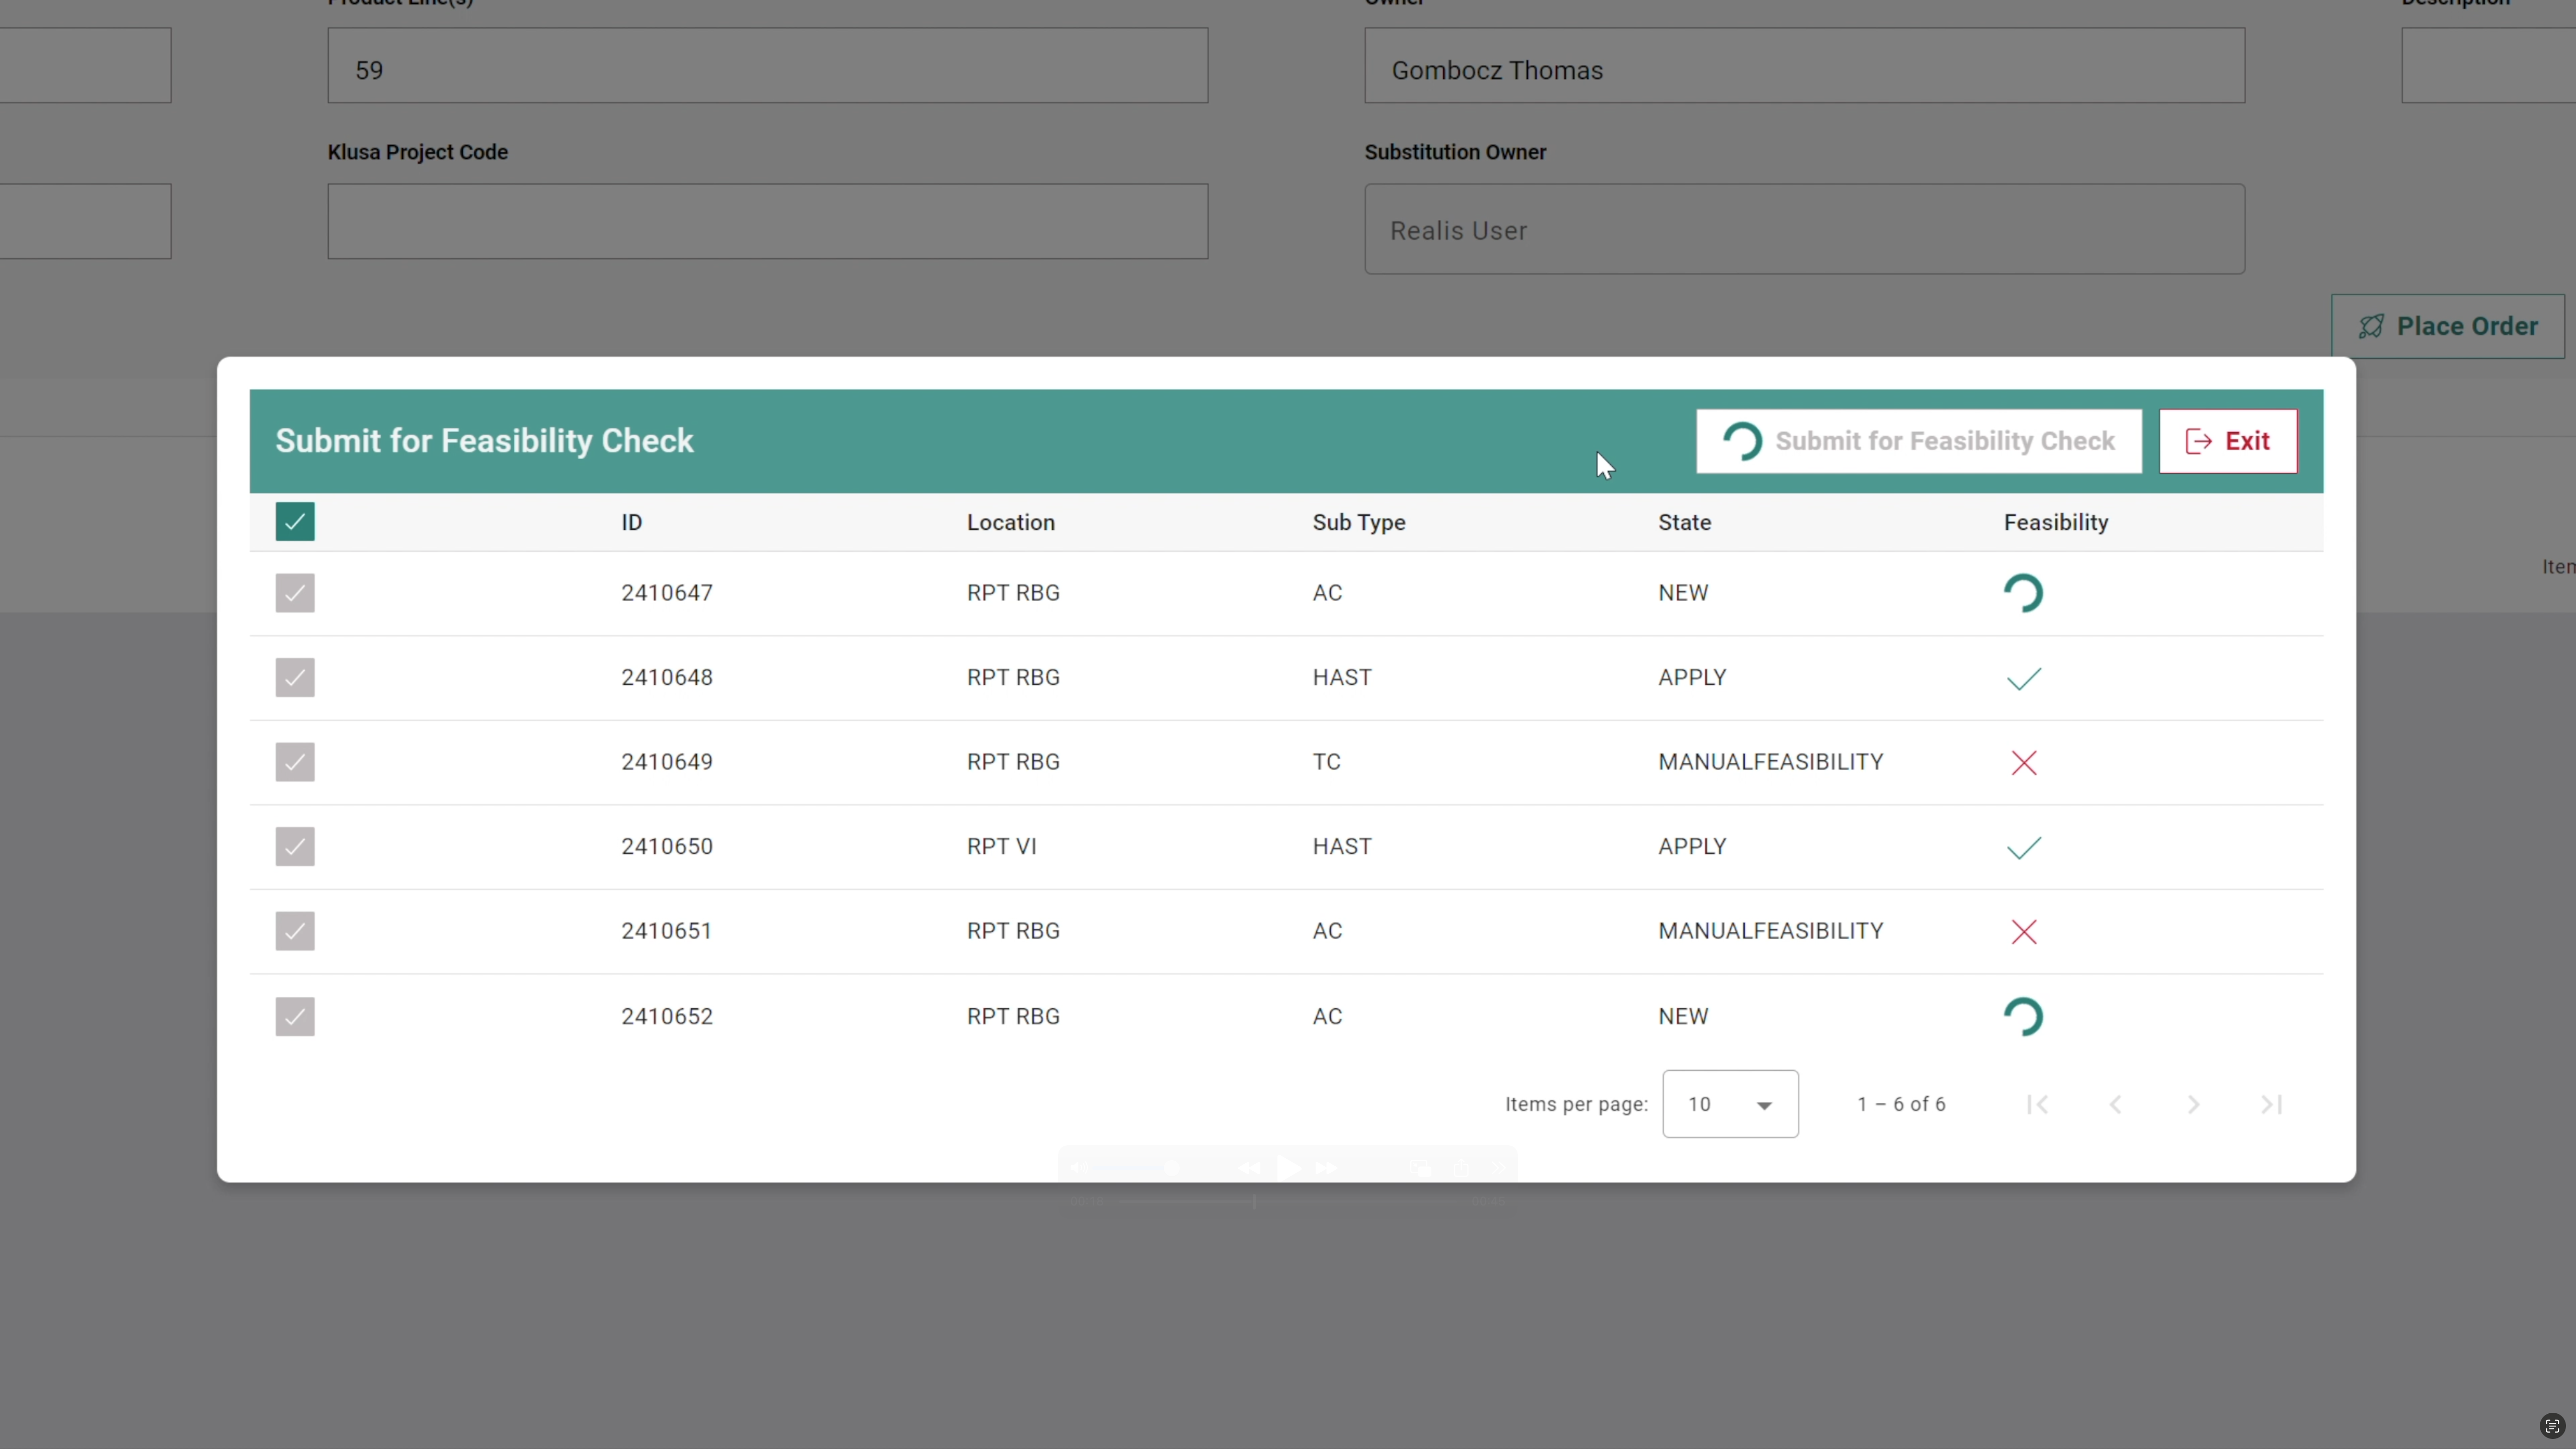
\includegraphics[width=0.85\paperwidth]{bilder/frontend/loading-with-results.png}} 
    \caption{Modal-Page ''Submit for Feasibility Check'' – Ladevorgang und erste Ergebnisse} 
    \label{fig:loading-with-results} 
\end{figure}

Sobald die ersten Überprüfungen abgeschlossen sind, verschwindet der Ladekreis. Anschließend werden drei Icons angezeigt und der Test-Status in der Tabelle aktualisiert.

Ein grüner Haken zusammen mit dem Status ''APPLY'' (bzw. „FEASIBLE“) signalisiert, dass der Feasibility Check erfolgreich war.

Ein rotes Kreuz und der Status ''MANUALFEASIBILITY'' weisen darauf hin, dass entweder ein oder mehrere Kriterien nicht erfüllt wurden oder der Test in der Konfiguration noch nicht für die automatisierte Überprüfung freigeschaltet ist. In beiden Fällen muss der Test manuell von einem Mitarbeiter überprüft werden.

Tritt ein Fehler im Algorithmus auf, erscheint ein rotes Dreieck mit Ausrufezeichen. In diesem Fall bleibt der Test-Status unverändert oder wird auf ''FEASIBILITY\_REQUEST'' gesetzt, je nachdem wann und welcher Fehler auftritt (dieser Fall ist in der Abbildung \ref{fig:loading-with-results} nicht dargestellt).


\subsection{Modal-Page für detaillierte Ergebnisse des Feasibility Checks}

Nachdem der Feasibility Check für einige Tests abgeschlossen ist, können in einer zweiten Modal-Page detaillierte Ergebnisse eingesehen werden. Diese Seite wird geöffnet, wenn der Benutzer den grün umrandeten „Show Feasibility“-Button in der Startoberfläche (siehe Abbildung \ref{fig:whole-page}) betätigt. Abbildung \ref{fig:result-details} zeigt diese Modal-Page.

\begin{figure}[!htbp] 
    \centering 
    \makebox[\textwidth]{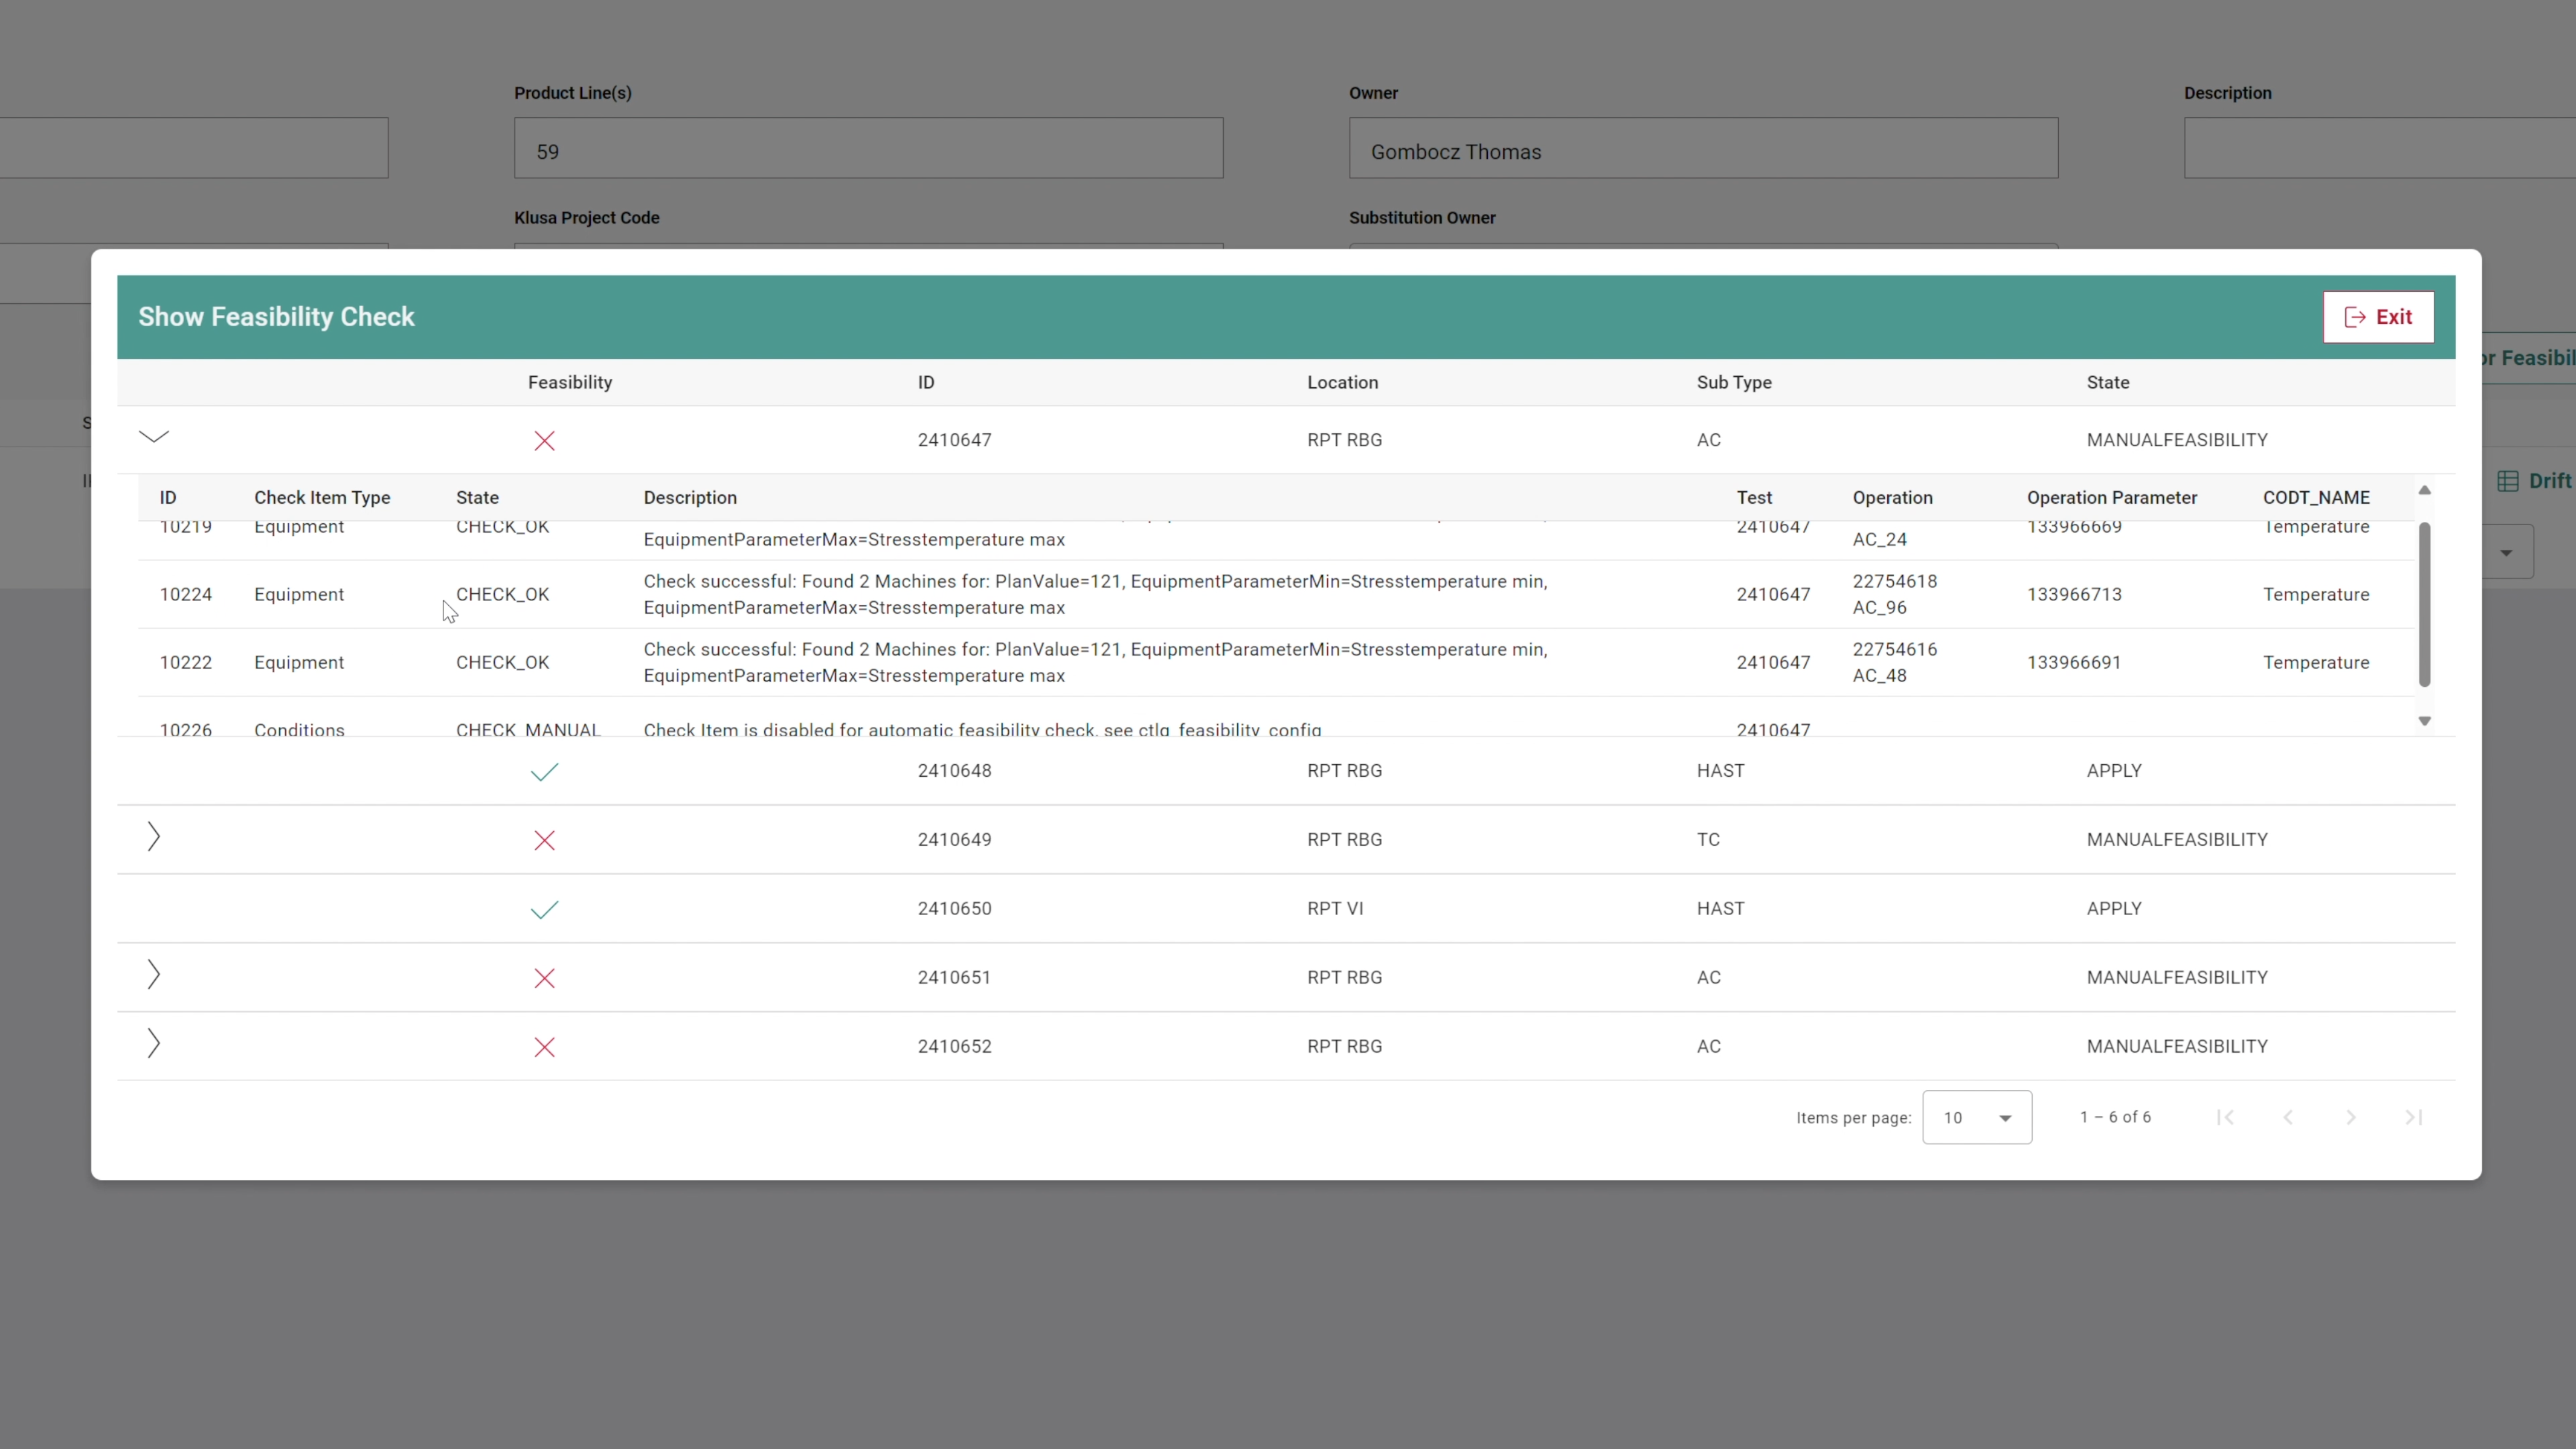
\includegraphics[width=0.85\paperwidth]{bilder/frontend/result-details.png}} 
    \caption{Modal-Page ''Submit Feasibility'' – Detaillierte Ergebnisse des Feasibility Checks} 
    \label{fig:result-details} 
\end{figure}

Das Popup-Fenster zeigt eine Tabelle mit allen Tests, ihren Informationen und den zugehörigen Ergebnissen. Der Benutzer kann einzelne Testzeilen aufklappen, um weitere Details zu erhalten. Links in der Tabelle sind Icons zu sehen, die anzeigen, welche Zeilen aufgeklappt werden können und welche aktuell geöffnet sind – dabei kann immer nur eine Zeile gleichzeitig ausgeklappt werden. 

In der aufgeklappten Ansicht werden in tabellarischen Form die gespeicherten \texttt{feasibility\_check\_item\_results}, des zugehörigen Tests angezeigt. Bei Tests die nur Überprüfungen mit dem Status-Ergebnis \texttt{''CHECK\_OFF''} aufweisen, liefern keine zusätzlichen Details, da in diesem Fall keine Feasibility-Resultate abgespeichert wurden. 

In der Spalte ''Check Item Type'' wird angegeben, ob es sich um einen Condition- oder Equipment Check handelt. In der Spalte ''State'' erscheint der Status, wie er in der Backend-Logik als Enum definiert ist. Zudem wird eine Beschreibung angezeigt, die dem Benutzer detaillierte Informationen zum jeweiligen Check liefert. Falls vorhanden, werden auch der zugehörige Operationstyp und die Parameter-ID dargestellt.

Diese Informationen sollen dem Benutzer helfen, die Ergebnisse nachvollziehen zu können. Außerdem ermöglichen sie es, bei unerwünschten Resultaten entsprechend zu reagieren. Entweder können die geplanten Tests und deren Parameter(-Werte) angepasst werden, oder weitere vom Feasibility Check abhängige Konditionen, wie etwa die Konfigurationstabelle können verändert werden.


